
\section{Experiments}\label{Experiments}

\subsection{Experimental Settings}

\begin{table*}[!htbp]
\centering
% \small
\setlength{\tabcolsep}{5.5pt}
\begin{tabular}{l|cc|cc|cccc|c}
\toprule
\multirow{2}{*}{\textbf{Method}} & \multicolumn{2}{c|}{\cellcolor{red!12}\textbf{PersonaMem}} & \multicolumn{2}{c|}{\cellcolor{blue!12}\textbf{PrefEval}} & \multicolumn{4}{c|}{\cellcolor{orange!12}\textbf{PersonaBench (Noise Level)}} & \cellcolor{cvprblue!20} \\
 & \cellcolor{red!12}32K & \cellcolor{red!12}128K & \cellcolor{blue!12}Explicit & \cellcolor{blue!12}Implicit & \cellcolor{orange!12}w/o Noise & \cellcolor{orange!12}0.3 & \cellcolor{orange!12}0.5 & \cellcolor{orange!12}0.7 & \multirow{-2}{*}{\cellcolor{cvprblue!20}\textbf{Overall}} \\ 
\midrule
Long Context & 34.36 & 25.05 & 31.70 & 30.80 & 29.00 & 19.10 & 17.83 & 13.00 & 26.90 \\
RAG          & 48.67 & 38.90 & 47.80 & 32.40 & 29.09 & 28.16 & 24.31 & 23.00 & 36.68 \\
\midrule
Mem0         & 48.53 & 39.67 & 57.60 & 46.40 & 17.60 & 19.75 & 19.22 & 17.80 & 38.23 \\
A-Mem        & 48.26 & 38.22 & 62.30 & 52.80 & 30.32 & 28.56 & 25.19 & 24.45 & 42.64 \\
LightMem     & 50.72 & 39.93 & 64.20 & 54.80 & 19.08 & 18.74 & 19.65 & 17.80 & 41.21 \\
\midrule
MemAgent     & 53.58 & 43.59 & 72.30 & 63.60 & 20.05 & 19.36 & 16.51 & 17.92 & 45.00 \\
Mem-$\alpha$ & 53.37 & 42.86 & 71.90 & 62.50 & 19.92 & 17.02 & 16.43 & 15.59 & 44.19 \\
\textbf{\ourmodel(Ours)} & \textbf{57.06} & \textbf{47.24} & \textbf{81.30} & \textbf{69.90} & \textbf{32.27} & \textbf{29.89} & \textbf{25.99} & \textbf{25.09} & \textbf{52.02} \\
\bottomrule
\end{tabular}
\caption{\textbf{Overall comparison across eight evaluation settings.} We report results on PersonaMem (32K/128K) (In-Domain), PrefEval (Explicit/Implicit) (Out-of-Domain), and PersonaBench under different noise levels (Out-of-Domain). Higher is better. The best results are highlighted in \textbf{bold}.}
% \vspace{-1em}
\label{tab:overall_eval}
\end{table*}


\textbf{Datasets and Metrics.}
We evaluate on three personalization memory benchmarks: {PersonaMem}~\cite{personamem}, {PrefEval}~\cite{prefeval}, and {PersonaBench}~\cite{tan2025personabench}. {PersonaMem} measures preference evolution over long multi-session histories at different context scales. PrefEval emphasizes explicit vs.\ implicit preference multi-choice queries (1{,}000 each) with 50 inserted turns. PersonaBench tests personalized retrieval and QA over heterogeneous, noisy user corpora. We report accuracy on PersonaMem and PrefEval, and F1 on PersonaBench. Details are reported in Appendix \ref{app:Datasets}.

\textbf{Baselines.}
We compare our approach against a diverse set of baselines.
\textbf{LongContext} directly feeds as much of the raw interaction history.
\textbf{RAG} denotes a retrieval-augmented generation setup that indexes all historical dialogue snippets in a vector store and retrieves the top-$K$ relevant segments.
To study external memory architectures, we further include three retrieval-based memory methods, \textbf{Mem0}, \textbf{A-Mem}, and \textbf{LightMem}, which maintain an external memory bank and update it.
We also compare with two reinforcement-learning-based memory agents, \textbf{MemAgent} and \textbf{MEM-$\alpha$}, which explicitly learn memory evolution actions.
All baselines are implemented on top of the same backbone and evaluated under the same data split and hyperparameter setup for a fair comparison.

\colorlet{pruneA}{orange!5} 
\colorlet{pruneB}{orange!10} 
\colorlet{pruneC}{red!12} 
\colorlet{pruneD}{red!15} 
\colorlet{pruneE}{red!20} 
\colorlet{pruneF}{red!25}
\begin{table}[t]
\centering
\small
\setlength{\tabcolsep}{1pt} % manual spacing only
\begin{tabular}{p{1.6cm}|M{1.4cm}M{1.4cm}|M{1.4cm}M{1.4cm}}
\toprule
\multirow{2}{*}{\textbf{Setting}} &
\multicolumn{2}{c|}{\textbf{PersonaMem}} &
\multicolumn{2}{c}{\textbf{PrefEval}} \\
& \textbf{32K} & \textbf{128K} & \textbf{Explicit} & \textbf{Implicit} \\
\midrule
\rowcolor{pruneF}\ourmodel          & \textbf{57.06} & \textbf{47.24} & \textbf{81.30} & \textbf{69.90} \\
\rowcolor{pruneE}w/o CF    & 56.44 & 46.33 & 78.30 & 68.10 \\
\rowcolor{pruneD}w/o GR       & 56.24 & 46.06 & 79.50 & 68.30 \\
\rowcolor{pruneC}w/o MGI    & 54.81 & 44.50 & 73.20 & 63.60 \\
\rowcolor{pruneB}w/o GMPO & 53.37 & 43.97 & 77.40 & 66.20 \\
\rowcolor{pruneA}w/o ALL         & 48.47 & 39.09 & 71.70 & 60.60 \\
\bottomrule
\end{tabular}
\caption{\textbf{Ablation Study.} \textbf{CF}: a contrastive feedback for textual-gradient guideline induction. \textbf{GR}: a guideline reward for enforcing the induced schema during memory updates.}
\vspace{-1em}
\label{tab:ablation}
\end{table}


\textbf{Implementation Details.}
We mainly leverage \texttt{Qwen2.5-7B-Instruct} \cite{yang2024qwen2} as the backbone LLM for all methods (\textsc{Mem-$\alpha$}  uses \texttt{Qwen3-4B}). For retrieval, we adopt \texttt{all-MiniLM-L6-v2}~\cite{wang2020minilm} and retrieve the Top-10 candidates. We construct training data by sampling 300 examples from PersonaMem. During training, we use retrieved dialogues as context to reduce computation when learning memory evolution; during inference, we feed the full dialogue history as context. Each memory-evolving round inputs a 4K-token chunk. All baselines are implemented using their publicly available codebases. For a fair comparison, MemAgent and MEM-$\alpha$ use their publicly released checkpoints, additionally training the same 300 PersonaMem training samples used by our method. All experiments are conducted on four A6000 GPUs. The same hyperparameters are shared across all retrieval-based methods. Hyperparameters are reported in Appendix~\ref{app:hyperparameter}.



\begin{figure}[ht]
\centering
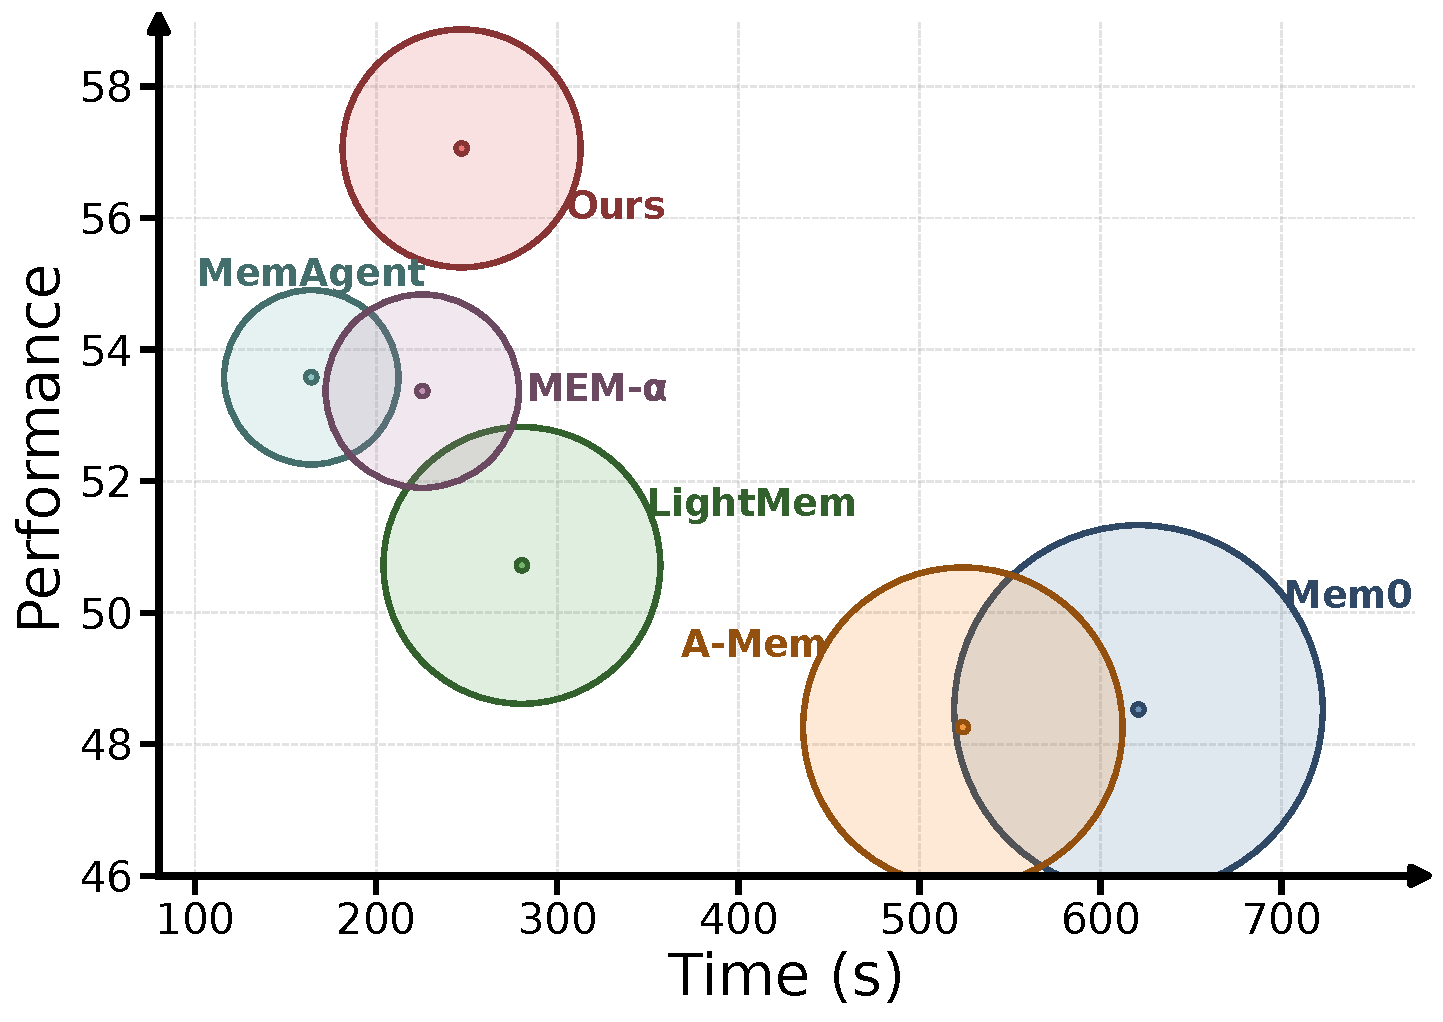
\includegraphics[width=0.88\linewidth]{img/efficiency_tradeoff.pdf}
\caption{Efficiency analysis on PersonaMem. We report the performance--time balance of memory construction/evolution over 20 dialogue histories (32K), where circle size indicates the standard deviation of runtime.}
\vspace{-1em}
\label{fig:efficiency_tradeoff}
\end{figure}

\subsection{Overall Evaluation}
\label{subsec:overall_eval}

\paragraph{Overall Comparison with Baselines.}
Table~\ref{tab:overall_eval} shows that \ourmodel achieves the best overall score across the three benchmarks, indicating that learning a memory-evolution mechanism is more effective than fixed context inclusion or manually designed update heuristics. Specifically, Long Context degrades notably under noisy histories, while \ourmodel captures user preference by filtering irrelevant content when evolving memory. 
Compared with explicit memory-bank baselines (Mem0, A-Mem, LightMem), \ourmodel delivers larger improvements on both PersonaMem and PrefEval. RL-based memory agents (MemAgent, Mem-$\alpha$) are competitive, yet they still lag behind in overall performance. This trend aligns well with our two-stage design: \moduleone induces a transferable guideline for memory evolution, while \moduletwo learns to retain preference-relevant information under the guideline, which demonstrates the effectiveness of our method for stable long-horizon personalization.
\paragraph{Generalizations Across Settings.}
Across the eight settings in Table~\ref{tab:overall_eval}, \ourmodel shows strong generality, consistently outperforming baselines on both in-domain tasks (PersonaMem, 32K$\rightarrow$128K) and out-of-domain tasks (PrefEval Explicit/Implicit; PersonaBench with increasing noise) evaluations, consistent with our two-stage design: \moduleone learns stable memory organizations, while \moduletwo retains preference-relevant information. We reported results in different categories in Appendix \ref{app:ComparisoninDifferentCategories}.



\begin{table}[t]
\centering
\small
\setlength{\tabcolsep}{5pt}
% \renewcommand{\arraystretch}{1} %可以控制行间距
\begin{tabular}{l|c c c c}
\toprule
\textbf{Method} & \makecell{\textbf{Qwen2.5-7B}\\\textbf{Instruct}}
& \makecell{\textbf{gpt-4o}\\\textbf{-mini}}
& \makecell{\textbf{gemini-2.5}\\\textbf{-flash}}
& \textbf{GPT-5} \\
\midrule
RAG & 48.67 & 47.44 & 61.15 & 63.80 \\
A-Mem & 48.26 & 48.47 & 62.37 & 64.42 \\
\midrule
 \multicolumn{5}{l}{\cellcolor{cvprblue!7}\textit{$\blacktriangledown$ Optimized w/ Qwen2.5-7B-Instruct}} \\
\ourmodel & \textbf{53.37} & 52.56 & 64.62 & 66.67 \\
\midrule 
 \multicolumn{5}{l}{\cellcolor{cvprblue!7}\textit{$\blacktriangledown$ Optimized w/ gpt-4o-mini}} \\
\ourmodel & 52.56 & \textbf{54.19} & \textbf{64.83} & \textbf{67.28} \\
\bottomrule
\end{tabular}
\caption{Cross-LLM transferability of \moduleone optimized guidelines (without RL). We optimize the guideline with one LLM and evaluate with different LLMs.}
\vspace{-1em}
\label{tab:cross_llm_transfer_textgrad}
\end{table}


\subsection{Ablation Study}

To further investigate the impact of each designed module, we conduct ablation study on two prevalent datasets. As depicted in Table~\ref{tab:ablation}, it shows that the full model performs best on both long-context PersonaMem and distractor-heavy PrefEval, indicating that our two-stage framework is necessary for stable memory evolution. Removing \textbf{CF} or \textbf{GR} causes consistent but smaller drops (e.g., PersonaMem 32k: 57.06$\rightarrow$56.44 / 56.24; PrefEval Explicit: 81.30$\rightarrow$78.30/79.50), suggesting that contrastive textual feedback and guideline-aligned rewards both improve update reliability. In contrast, ablating either stage yields more significant degradations: removing \textbf{\moduleone} most strongly hurts preference retention and inference performance (PrefEval Explicit/Implicit: 81.30/69.90$\rightarrow$73.20/63.60), while removing \textbf{\moduletwo} more severely impacts long-horizon tracking on PersonaMem (32k/128k: 57.06/47.24$\rightarrow$53.37/43.97). Finally, \textbf{w/o ALL} collapses performance across benchmarks (PersonaMem 32k: 48.47; PrefEval Explicit: 71.70), confirming that learned guidelines plus guideline-aligned policy optimization are both critical.



\subsection{Efficiency Analysis}

Considering the use of LLMs, we further explore the efficiency of our proposed method. Figure~\ref{fig:efficiency_tradeoff} illustrates the performance-time trade-off of memory construction/evolution. Our \ourmodel achieves the best performance while remaining among the faster approaches, indicating a favorable efficiency frontier rather than a pure accuracy-at-any-cost gain. This advantage is consistent with the design of \ourmodel: instead of repeatedly invoking an LLM to separately extract and merge memory entries (e.g., A-Mem and Mem0), our approach \textbf{internalizes extraction, update, and forgetting behaviors into the model’s memory evolution process}, reducing integration overhead. In contrast, MemAgent and MEM-$\alpha$ run quickly but fall behind in performance, suggesting that their memory update mechanism cannot reliably maintain useful user information.


\subsection{Cross-LLM Transferability of Guidelines}

We also investigate the transferability of different LLMs in our method, particularly focusing on the LLMs used for optimization and evaluation. As shown in Table~\ref{tab:cross_llm_transfer_textgrad}, we select various mainstream LLMs to evaluate whether \textbf{optimized guidelines} transfer across different backbone LLMs. The results show that, across all four LLMs, both \moduleone variants consistently outperform the baselines (RAG and A-Mem), indicating that the learned guideline captures model-agnostic memory-update principles rather than overfitting to a specific LLM. Notably, optimizing with \texttt{gpt-4o-mini} generalizes strongly and achieves the best numbers on three backbones, including \texttt{GPT-5} and \texttt{gemini-2.5-flash}. Overall, these results support that \moduleone produces a guideline that is portable across LLMs, making it practical to optimize once and deploy under different backbone choices.

\begin{figure}[t]
\centering
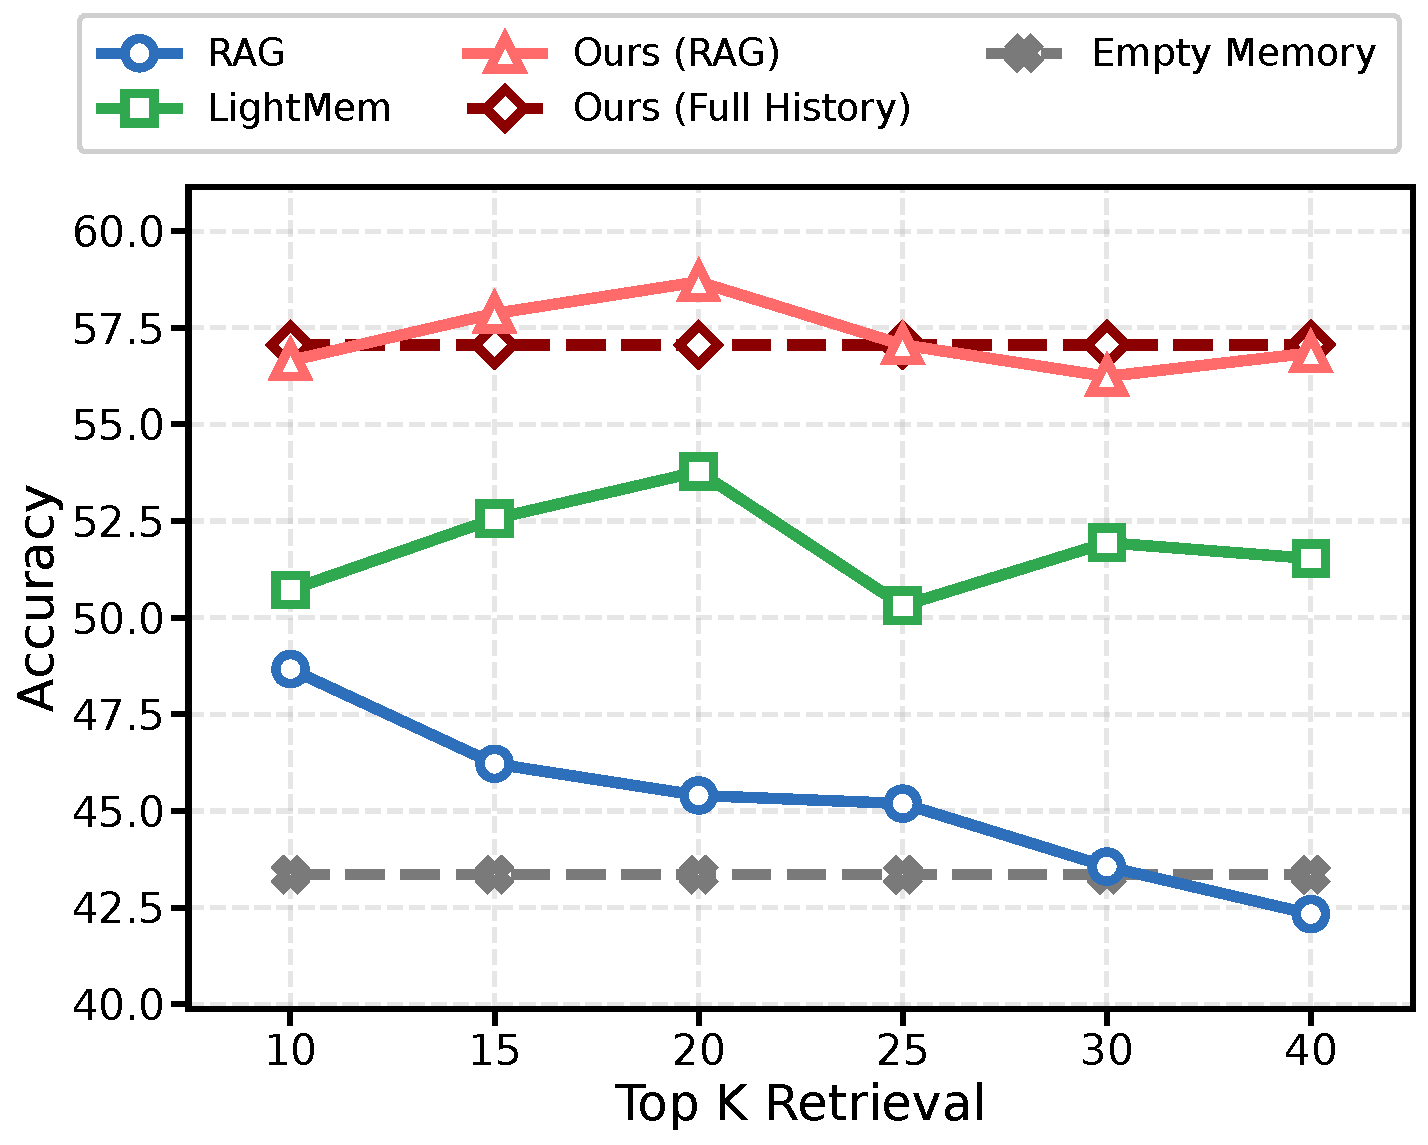
\includegraphics[width=0.9\linewidth]{img/topk_curve.pdf}
\caption{Retrieval Top-$K$ on PersonaMem (32K).}
\vspace{-1em}
\label{fig:topk}
\end{figure}



\subsection{Comparison on Different Retrieval}
% Figure~\ref{fig:topk} evaluates how performance changes as we vary the retrieval Top-$K$. 
In Figure~\ref{fig:topk}, we examine how Top-$K$ retrieval affects different methods on the PersonaMem dataset.
Across all Top-$K$, both inference modes of our approach (performing memory evolution on retrieved context, \textbf{Ours (RAG)}, or on full history, \textbf{Ours (Full History)}) remain consistently strong and clearly outperform the baselines.
Notably, \textbf{Ours (RAG)} peaks around $K{=}20$ and even surpasses the full-history variant, which suggests that retrieval can be beneficial when it filters irrelevant context and reduces noise for better memory evolution. In contrast, vanilla RAG degrades as $K$ increases and even drop below Empty Memory, indicating that simply adding more retrieved content may introduce distractors that hurt downstream decisions. Overall, these results show that retrieval is not sufficient on its own; it achieves its best effect when coupled with \ourmodel to transform retrieved evidence into coherent memory.



\subsection{Impact of Per-Round Token Budget on Memory Evolution}
\begin{figure}[t]
\centering
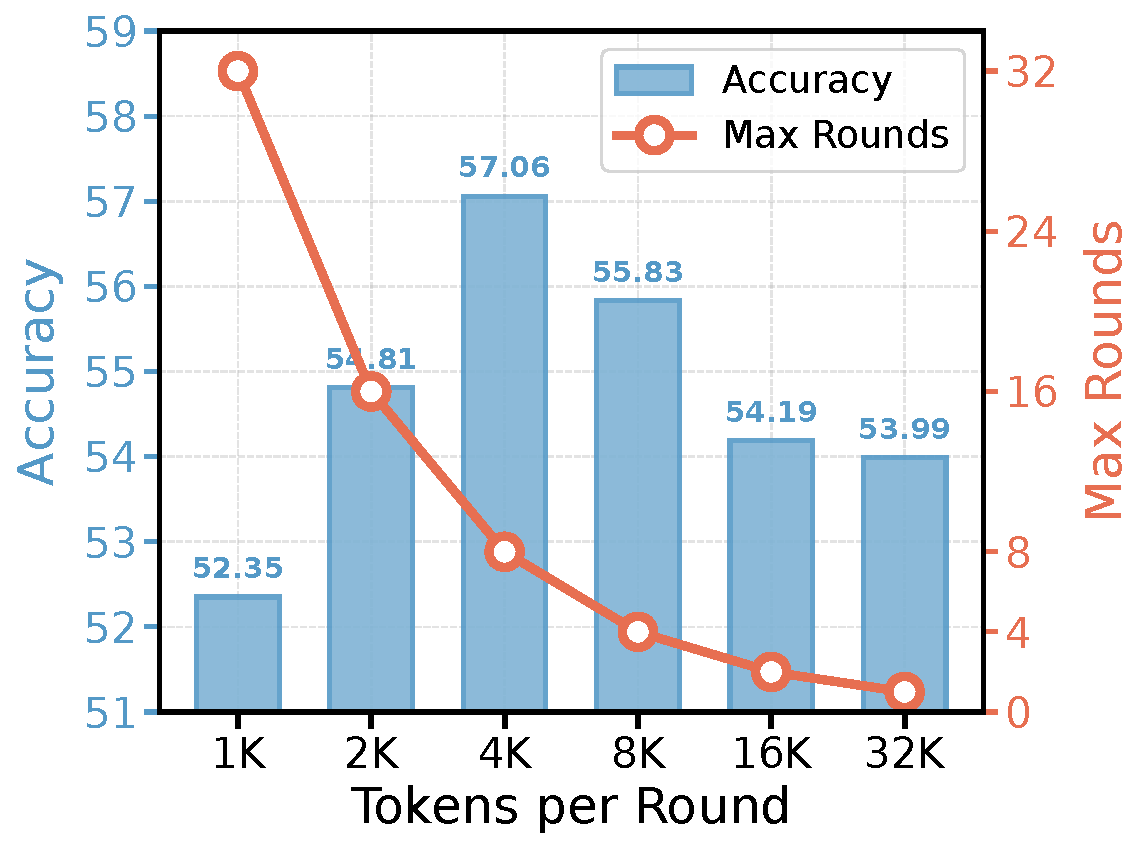
\includegraphics[width=0.98\linewidth]{img/dual_yaxis_tokens_rounds.pdf}
\caption{Effect of tokens per evolve round on PersonaMem (32K).}
\vspace{-1em}
\label{fig:tokens_rounds}
\end{figure}


% Figure~\ref{fig:tokens_rounds} analyzes how the per-round evolution token budget affects memory evolution. 
Since the per-round token budget directly determines inference cost in real-world deployment, we study its impact on memory evolution in Figure~\ref{fig:tokens_rounds}.
When token budget is too small (e.g., 1K--2K), system must split history into many rounds, and repeated evolve operations can accumulate errors and trigger uncontrolled forgetting, which ultimately hurts accuracy. In contrast, increasing budget initially tends to improve performance by reducing the required number of rounds and stabilizing the update dynamics. However, excessively large budgets (8K--32K) can make each evolution step more challenging, as the resulting context becomes more complex, thereby increasing the difficulty of processing information within a single pass. Overall, the results suggest a clear trade-off: effective memory evolution requires a moderate per-round token budget that avoids both excessive update frequency and overly complex single-step contexts.


\subsection{Effect of Guideline Quality}
Finally, to gain a more intuitive understanding of the impact of guideline quality, we compare guidelines of different quality levels.
As shown in Figure~\ref{fig:prompt}, improving the quality of the memory-update guideline consistently strengthens downstream performance. Starting from a manually written prompt, an LLM rewrite yields a moderate gain, suggesting that surface-level prompt refinement helps but remains limited. Note that, the guideline induced by \moduleone achieves the best results on both settings, reaching 53.28 on 32K and 43.76 on 128K, which corresponds to relative improvements of +10.4\% and +11.3\% over the manual prompt, respectively. The error bars across three seeds indicate that these gains are stable rather than driven by randomness.

\begin{figure}[t]
\centering
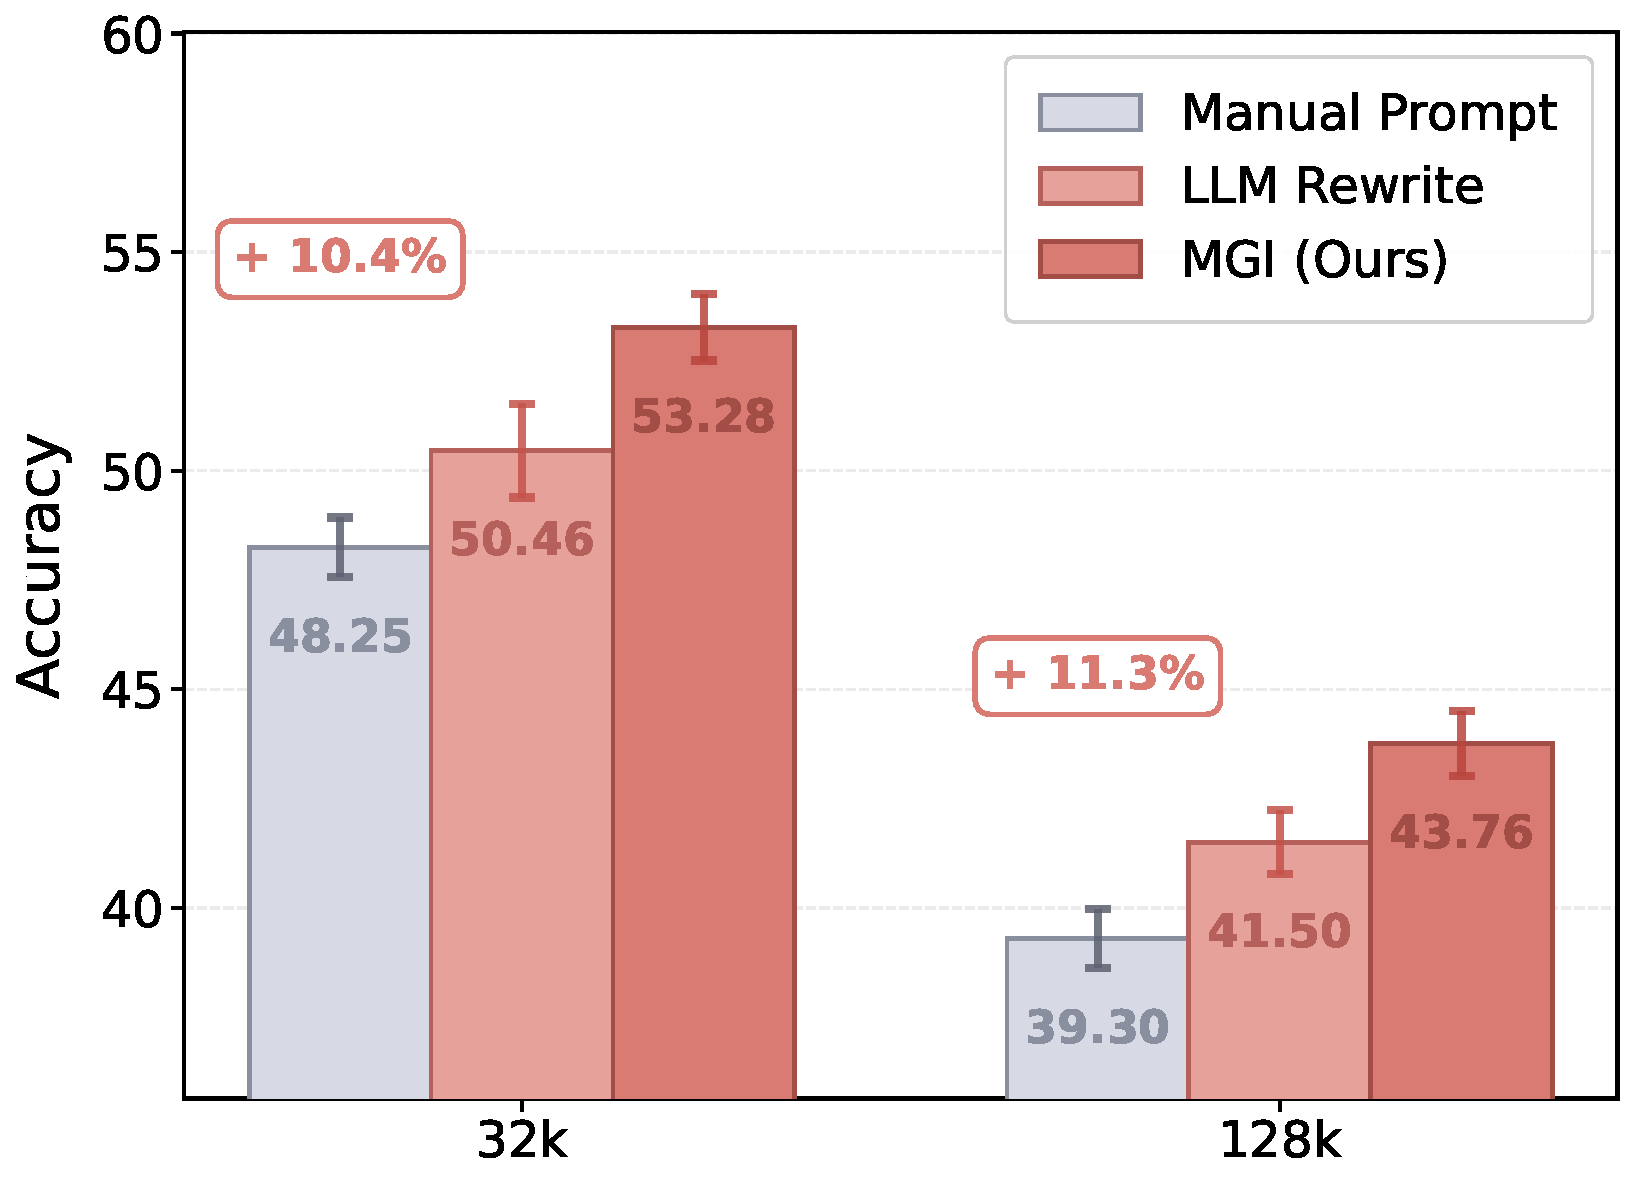
\includegraphics[width=0.89\linewidth]{img/prompt_bar.pdf}
\caption{Impact of prompt quality on PersonaMem, averaged over three random runs with different seeds; error bars indicate standard deviation.}
\vspace{-1em}
\label{fig:prompt}
\end{figure}
